%*****************************************
\chapter{Erste Vorüberlegungen}\label{ch:examples}
%*****************************************
Nachdem nun die theoretische Thematik ausgeführt wurde, ist es nun von Bedeutung, eine Möglichkeit zu finden diese anzuwenden. 
Um das Werkzeug der sozialen Netzwerkanalyse besser zu verstehen, ist es immer von Vorteil die eigenen Daten, die Social Media wie Twitter, Instagram und Facebook zur Verfügung stellen, zu interpretieren und sich daran zu erproben. 

Da Facebook und Instagram der Informationspflicht unterliegen, ist es sehr simpel die eigenen social Media Daten anzufordern. Diese ähneln sich von ihrem Aufbau und Inhalt enorm. Meist handelt es sich hier um die geliketen und kommentierten Posts der Nutzer*innen, verfasste Nachrichten und gesuchte Inhalte. Jedoch enthalten die Daten nicht sonderlich viele Inhalte die sich der Interpretation eignen. Diese beschränken sich meistens auf den Benutzernamen und einen sogenannten $"$Timestamp$"$, welcher nicht näher erklärt oder definiert ist, aber aus zehn Ziffern besteht.
Ein Grund, warum es nicht funktioniert hat, eine wissenschaftliche Arbeit über eigene Daten zu schreiben, war die Zusammensetzung der Graphen und die schnelle Einsicht meinerseits, dass es sich bei den erstellten Plots und Ergebnissen nicht um $"$soziale Netzwerke$"$ handeln kann.
Denn die Graphen bestanden zum größten Teil aus einzelnen Teilgraphen, welche nicht voneinander abhängig waren oder annähernd Zusammenhänge aufweisen konnten. Auch gab es keine Cliquen oder Bridgen (Brücken). \\
\FloatBarrier
\begin{figure}[h!]
    \centering
    %\hspace*{-1cm}
    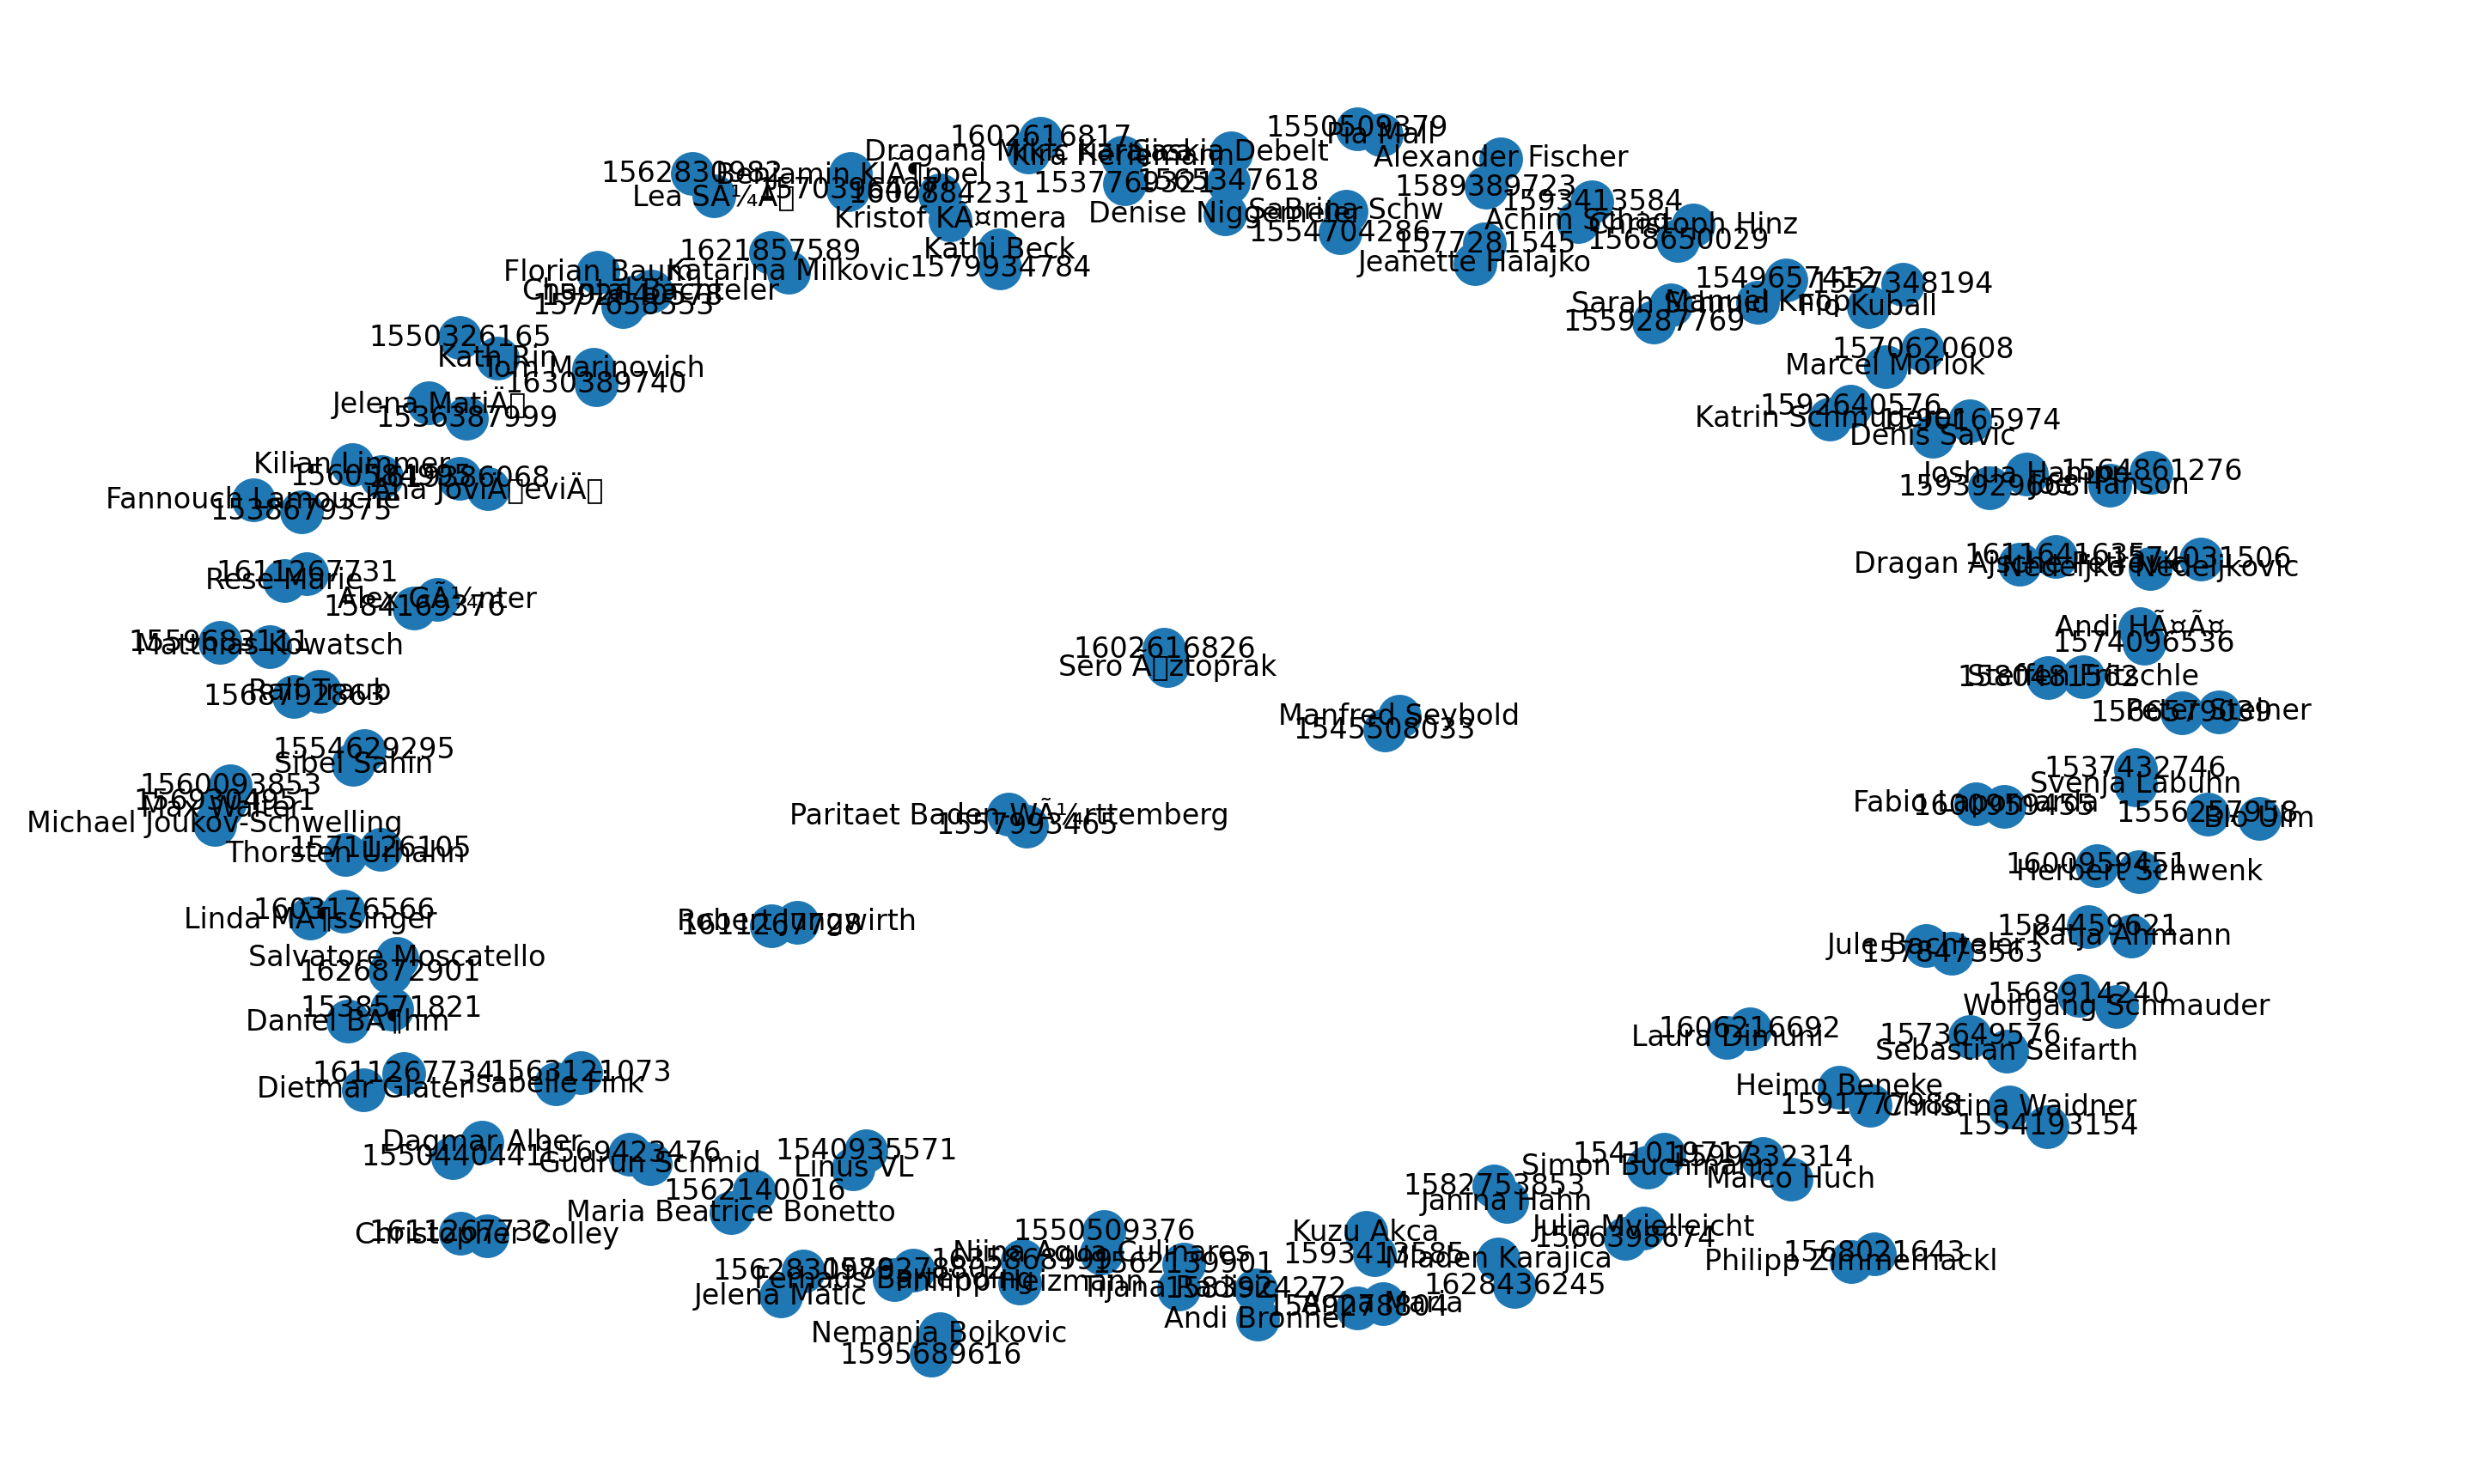
\includegraphics[width=0.9\textwidth]{Graphics/PlotOwnData.png}
    \caption{Erste Versuche eines Sozialen Netzwerks}
    \label{fig:OwnData}
\end{figure}
\FloatBarrier

Eine weitere Schwierigkeit war die Interpretation der Kanten, denn diese war zu valide. 
Auf den ersten Blick sahen die Graphen oft identisch aus, doch immer wieder kam die Frage auf, was die Knoten und was Beziehung zu den Kanten aussagen könnten. Handelt es sich hier um fixe, eindeutige zugeordnete IDs, die im Umkehrschluss auf die Kanten die Bedeutung $"besitzt"$ haben könnte.\\
Dementsprechend war das weitere Vorgehen mit eigenen Daten nicht zielführend und der Wunsch kam auf, eigene, zufällige Netzwerke zu generieren. 

\section{Generierung eines random Netzwerk-Plots} 
Bei einer endlichen Anzahl von Knoten n gibt es auch eine endliche Anzahl von Graphen, die aus diesen Knoten erzeugt werden können, auch wenn die Anzahl der Graphen mit n Knoten exponentiell wächst.
Ein Zufallsgraph ist nur einer dieser Graphen, der durch einen Zufallsprozess erzeugt wird.
Genauer gesagt gibt es eine Wahrscheinlichkeitsverteilung über alle möglichen Graphen, die beschreibt, wie wahrscheinlich jeder Graph durch den Zufallsprozess ausgewählt wird.
Wenn von $"$Zufallsgraphen$"$ die Rede ist, wird in den meisten Fällen in Python das zugrunde liegende "Erdős-Rényi-Modell" als Graphengenerator angenommen (benannt nach den Mathematikern Paul Erdős und Alfréd Rényi). Eine wichtige Eigenschaft von auf diese Art erzeugten Zufallsgraphen ist, dass bei einer Menge von Knoten und einer Anzahl von Kanten alle möglichen Graphen mit der gleichen Wahrscheinlichkeit erzeugt werden. Es gibt also keine Vorliebe für eine bestimmte Art von Graphen. Das heißt es handelt sich hierbei um eine Gleichverteilung.

\begin{itemize}
    \item der Erdős-Rényi-Graphengenerator Algorithmus beginnt mit n unverbundenen Knoten.
    \item Gehe jede mögliche Kante e durch. Nimm dann die Kante e mit einer (unabhängigen) Wahrscheinlichkeit p in den Graphen auf
    \item Die Laufzeit des Algorithmus ist $n \times n$ mögliche Kanten gibt, ist die Laufzeit $O(n^2)$
    \item alle Graphen haben die gleiche Wahrscheinlichkeit
    \item es gibt zwei Parameter für den Algorithmus: die Anzahl der Eckpunkte n und die Anzahl der Kanten e.
\end{itemize}

Aber neben dem Erdős-Rényi-Modell, gibt es noch viele weitere Methoden zur random Netzwerkmodellierung mit Python. In der ersten Version haben wir $n = 25$ gewählt, wobei $n$ die Anzahl der Knoten ist.
\begin{itemize}
    \item die $"$ dense$\_$gnm$\_$random$\_$graph$"$ Modellierung verwendet. Dieser liefert einen $G_{n,m}$-Zufallsgraphen.
    Beim $G_{n,m}$-Modell wird ein Graph gleichmäßig zufällig aus der Menge aller Graphen mit $n$ Knoten und $m$ Kanten ausgewählt.
    \item die $"$Newman–Watts–Strogatz small-world graph$"$-Modellierung verwendet. Die funktioniert wie folgt: \\
    Zunächst wird ein Ring mit $n$ Knoten erzeugt. Dann wird jeder Knoten im Ring mit seinen $k$ nächsten Nachbarn verbunden (oder $k - 1$ Nachbarn, wenn $k$ ungerade ist). Dann werden Abkürzungen durch Hinzufügen neuer Kanten wie folgt erstellt: \\
    Für jede Kante $(u, v)$ im zugrundeliegenden $"$ $n$-Ring mit $k$ nächsten Nachbarn$"$ wird mit der Wahrscheinlichkeit $p$ eine neue Kante $(u, w)$ mit einem zufällig ausgewählten bestehenden Knoten w hinzugefügt. Im Gegensatz zu $"$watts$\_$strogatz$\_$graph()$"$ werden keine Kanten entfernt
    \item Die $"$random$\_$regular$\_$graph $"$-Modellierung Gibt einen zufälligen $d$-regulären Graphen mit $n$ Knoten zurück.
    Der resultierende Graph hat keine Selbstschleifen oder parallele Kanten
    \item Die $"$barabasi$\_$albert$\_$graph$"$-Modellierung hingegen liefert einen Zufallsgraphen nach dem Barabási-Albert-Präferenzmodell.
    Ein Graph mit $n$ Knoten wird durch Anhängen neuer Knoten mit jeweils $m$ Kanten erzeugt, die bevorzugt an bestehende Knoten mit hohem Grad angehängt werden.
    \item Die $"$powerlaw$\_$cluster$\_$graph$"$-Modellierung ist im wesentlichen das Barabási-Albert (BA)-Wachstumsmodell mit dem zusätzlichen Schritt, dass auf jede zufällige Kante eine Chance folgt, auch eine Kante zu einem seiner Nachbarn (und damit ein Dreieck) zu bilden. Dieser Algorithmus verbessert BA insofern, als er eine höhere durchschnittliche Clusterbildung ermöglicht, falls gewünscht.
\end{itemize}

\FloatBarrier
\begin{figure}[h!]
    \centering
    \hspace*{-1.5cm}
    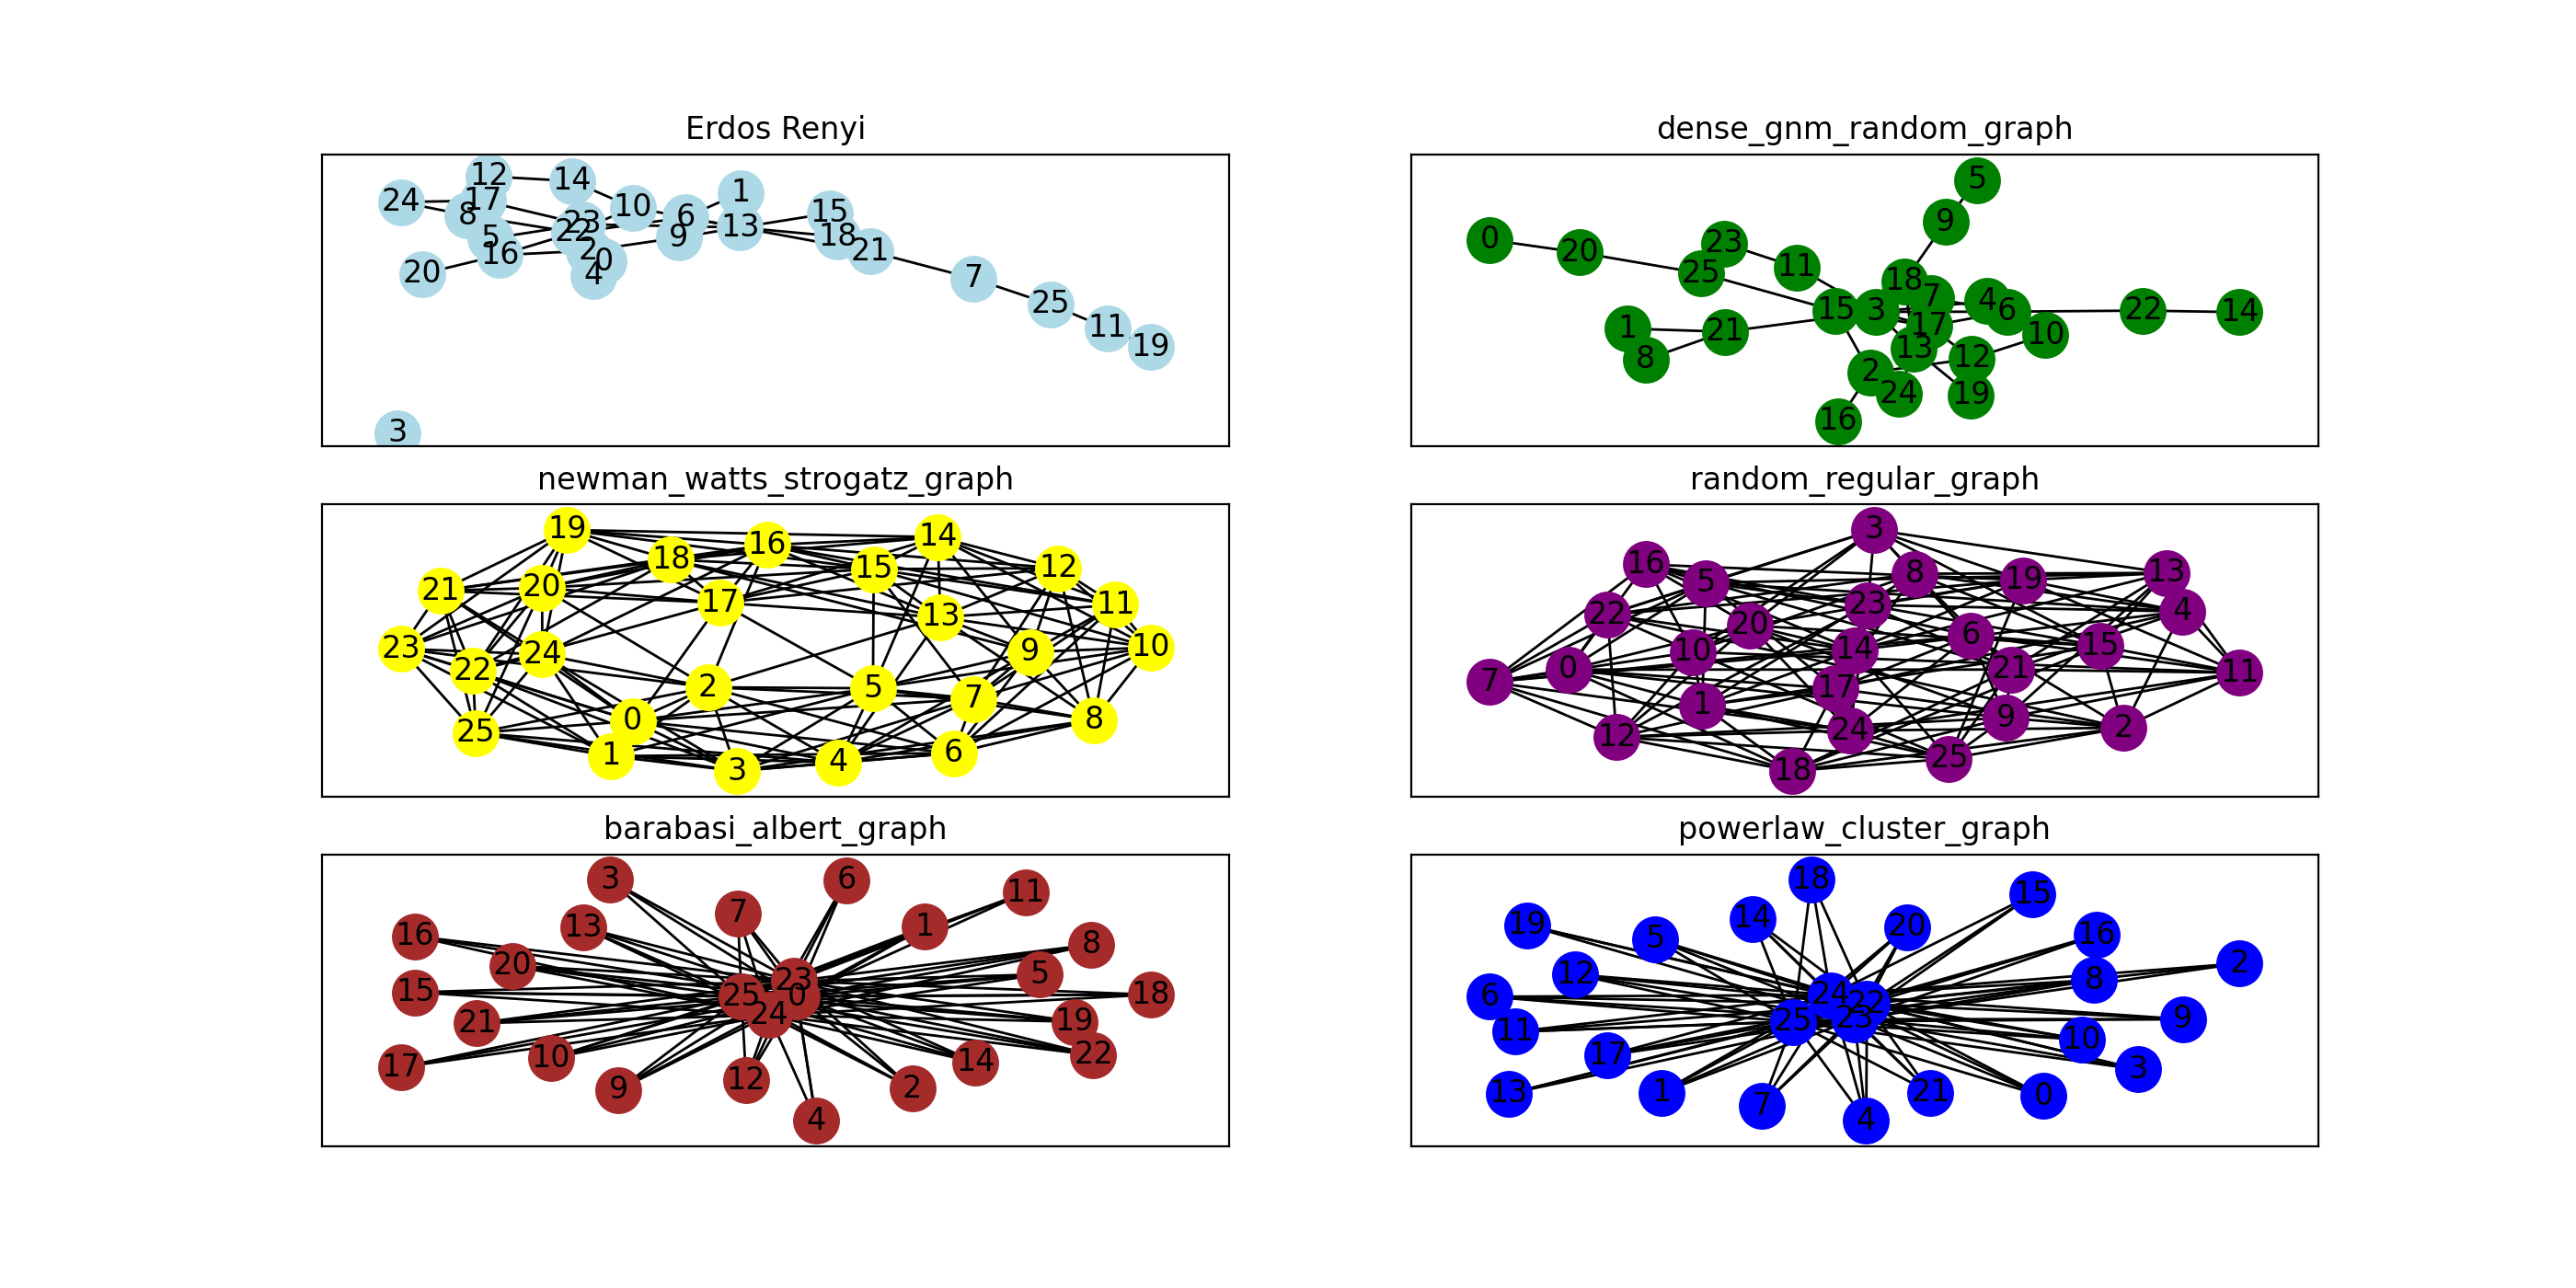
\includegraphics[width=1.2\textwidth]{Graphics/6Random.png}
    \caption{Random Graphen-Modellierung}
    \label{RandomGraphen}
\end{figure}

\newpage
Isolation bedeutet im Social Network Zusammenhang, dass ein Knoten keinen Nachbarn besitzt (Grad $0$ aufweist).
Für gerichtete Graphen heißt dies, dass es keine in- und out-Nachbarn gibt. Dies würde auf Soziale Netzwerke, beziehungsweise Sozial Media, bezogen bedeuten, dass Nutzer*innen auf dieser Plattform existieren, die keinerlei Verbindungen nachweisen können. Dies kann durchaus der Fall sein, aber doch ist es sehr unwahrscheinlich, dass Menschen auf solchen Plattformen angemeldet sind und keinerlei Freunde haben oder andere Nutzer*innen kennen mit denen eine Verbindung besteht. Bei der Interpretation wäre es sogar möglich, einen Schritt weiter zu gehen. Eine Person, welche keiner weiteren Person folgt oder mit dieser Befreundet ist und der selbst keine Personen folgen, könnte eine fiktive Person sein. Denn solche Plattformen zielen darauf ab, Menschen miteinander zu verbinden und auch über räumlich große Distanzen hinweg in Verbindung zu halten. Daher muss auch bei diesem Vorgehen kritisch hinterfragt werden, ob es sich bei den Graphen um soziale Netzwerke handelt. Die Vermutung liegt nahe, dass es bei den Werten um fehlerhafte Zentralitäten handelt, jedoch kann dies noch optimiert werden.
Die sozialen Graphen, die mit diesen Methoden entstanden sind, sehen wir in Abbildung \ref{RandomGraphen}. Doch auch hier war keine ansprechend genug. Noch am ehesten entspricht das Erdős-Rényi Modell einem sozialen Graph, wenn wir ausschließlich die Form der Graphen betrachten. Die Analyse der Zentralitäts-Werten hat an dieser Stelle nicht weiter stattgefunden, da bereits das erste Kriterium, dass es mehrere Verzweigungen im Graphen gibt und dass nicht automatisch alle Knoten mit den anderen Knoten verbunden sind. Zudem waren die Ergebnisse der Zentralitäten teilweise unstimmig, fehlerhaft und würden im Rahmen dieser Arbeit zu Verwirrungen führen. Dementsprechend liegt nahe, dass wir hier eine weitere Anpassung durchführen müssen. Doch wie könnte eine Anpassung aussehen? 

\section{Random Graphen-Optimierung}
Eine mögliche Optimierung erzielen wir, indem wir von den Random Graphen-Methoden abweichen, welche Python den Nutzer*innen zur Verfügung stellt. Eine weitere Überlegung, um eine Optimierung zu erzielen, ist zudem alle Formeln selbständig zu implementieren und nicht die bereits vordefinierten Python-Funktionen zu verwenden. Zum einen sind diese vordefinierten Funktionen intransparent und da sie die Rückgabewerte im Datentyp $"$Dictionary$"$ ausgeben, wird es automatisch fehleranfälliger, auf diese korrekt zuzugreifen. Zudem erlangen wir dafür im Idealfall ein noch besseres Verständnis für die Formel. Zu einem späteren Zeitpunkt werden wir uns zudem ein Code-Ausschnitt anschauen.
Doch auch die Optimierung und Umstrukturierung bringt Schwierigkeiten mit sich. Begonnen mit der gewichteten Gradzentralität, hier ist es zunächst von Vorteil, die Datenstruktur genauer zu betrachten. Zunächst sind alle $edge\_labels$ als einzelne Items in einer Liste ausgeprintet um einen besseren Überblick über die Struktur zu bekommen. Die Struktur sieht folgendermaßen aus \\
$[((0, 2), 6), ((0, 4), 5)]$ wobei das Tupel die zwei Knoten beschreibt, zwischen denen eine Kante existiert (also in unserem Fall existiert zwischen den Knoten $0$ und $2$ eine Kante. Der Wert dahinter repräsentiert das Gewicht. Also in unserem Fall ist der existierenden Kante zwischen $0$ und $2$ das Gewicht $6$ zugeschrieben. Schnell fällt auf, dass wir den 2. Wert des Tupels nicht benötigen da für den Moment nicht relevant ist, wohin die Kante führt, aber dass sie aus dem Knoten entspringt ist durchaus relevant. Daher muss der von Python ausgeprintete Typ $"$Dictionary$"$ in eine Liste umgewandelt werden, bei den Tupeln der 2. Wert entfernt und anschließend der 1. Wert von dem Tupel mit den Gewichten der Kanten gegenübergestellt werden. Zum Schluss werden die Gewichte zusammengezählt, welche die gleiche Knoten-Nummer besitzen.\\ \todo{vielleicht anhand Beispiel genauer beschreiben was gemeint ist}
Bei der closeness centrality ergibt sich ein ganz analoges Problem. Die Werte scheinen nicht zu passen bei der von Python vordefinierten Funktion für gewichtete Graphen. Zunächst müssen die Graphen wieder ungerichtet sein, weil bei den Berechnungen aufgefallen ist, dass es bei gerichteten durchaus häufiger zu Fehlern kommt, weil die Gewichte stark variieren und bei den Berechnungen die Richtungen nicht eindeutig sind.
Bei weiteren Überlegungen ist die Idee entstanden, eine Methode zu schreiben, die sicherstellt, dass der ausgegebene Graph aus einer vorgegebenen Anzahl an Cliquen besteht. Hierbei ist ein Trick von Bedeutung. Der Methode wird eine fixe Zahl $n$ übergeben und sichergestellt, dass so lange die Anzahl an Cliquen nicht genau dieser fixen Zahl $n$ entspricht, stetig neue Graphen generiert werden müssen, bis letztendlich ein Graph generiert wurde, mit exakt $n$ Cliquen. Zudem wird eine Variable mit einem Wert $k$ übergeben welche auch die Größe der Cliquen festlegen kann. Entstanden ist folgendes Zwischenergebnis:
\FloatBarrier
\begin{figure}[h!]
    \centering
    \hspace*{-1.5cm}
    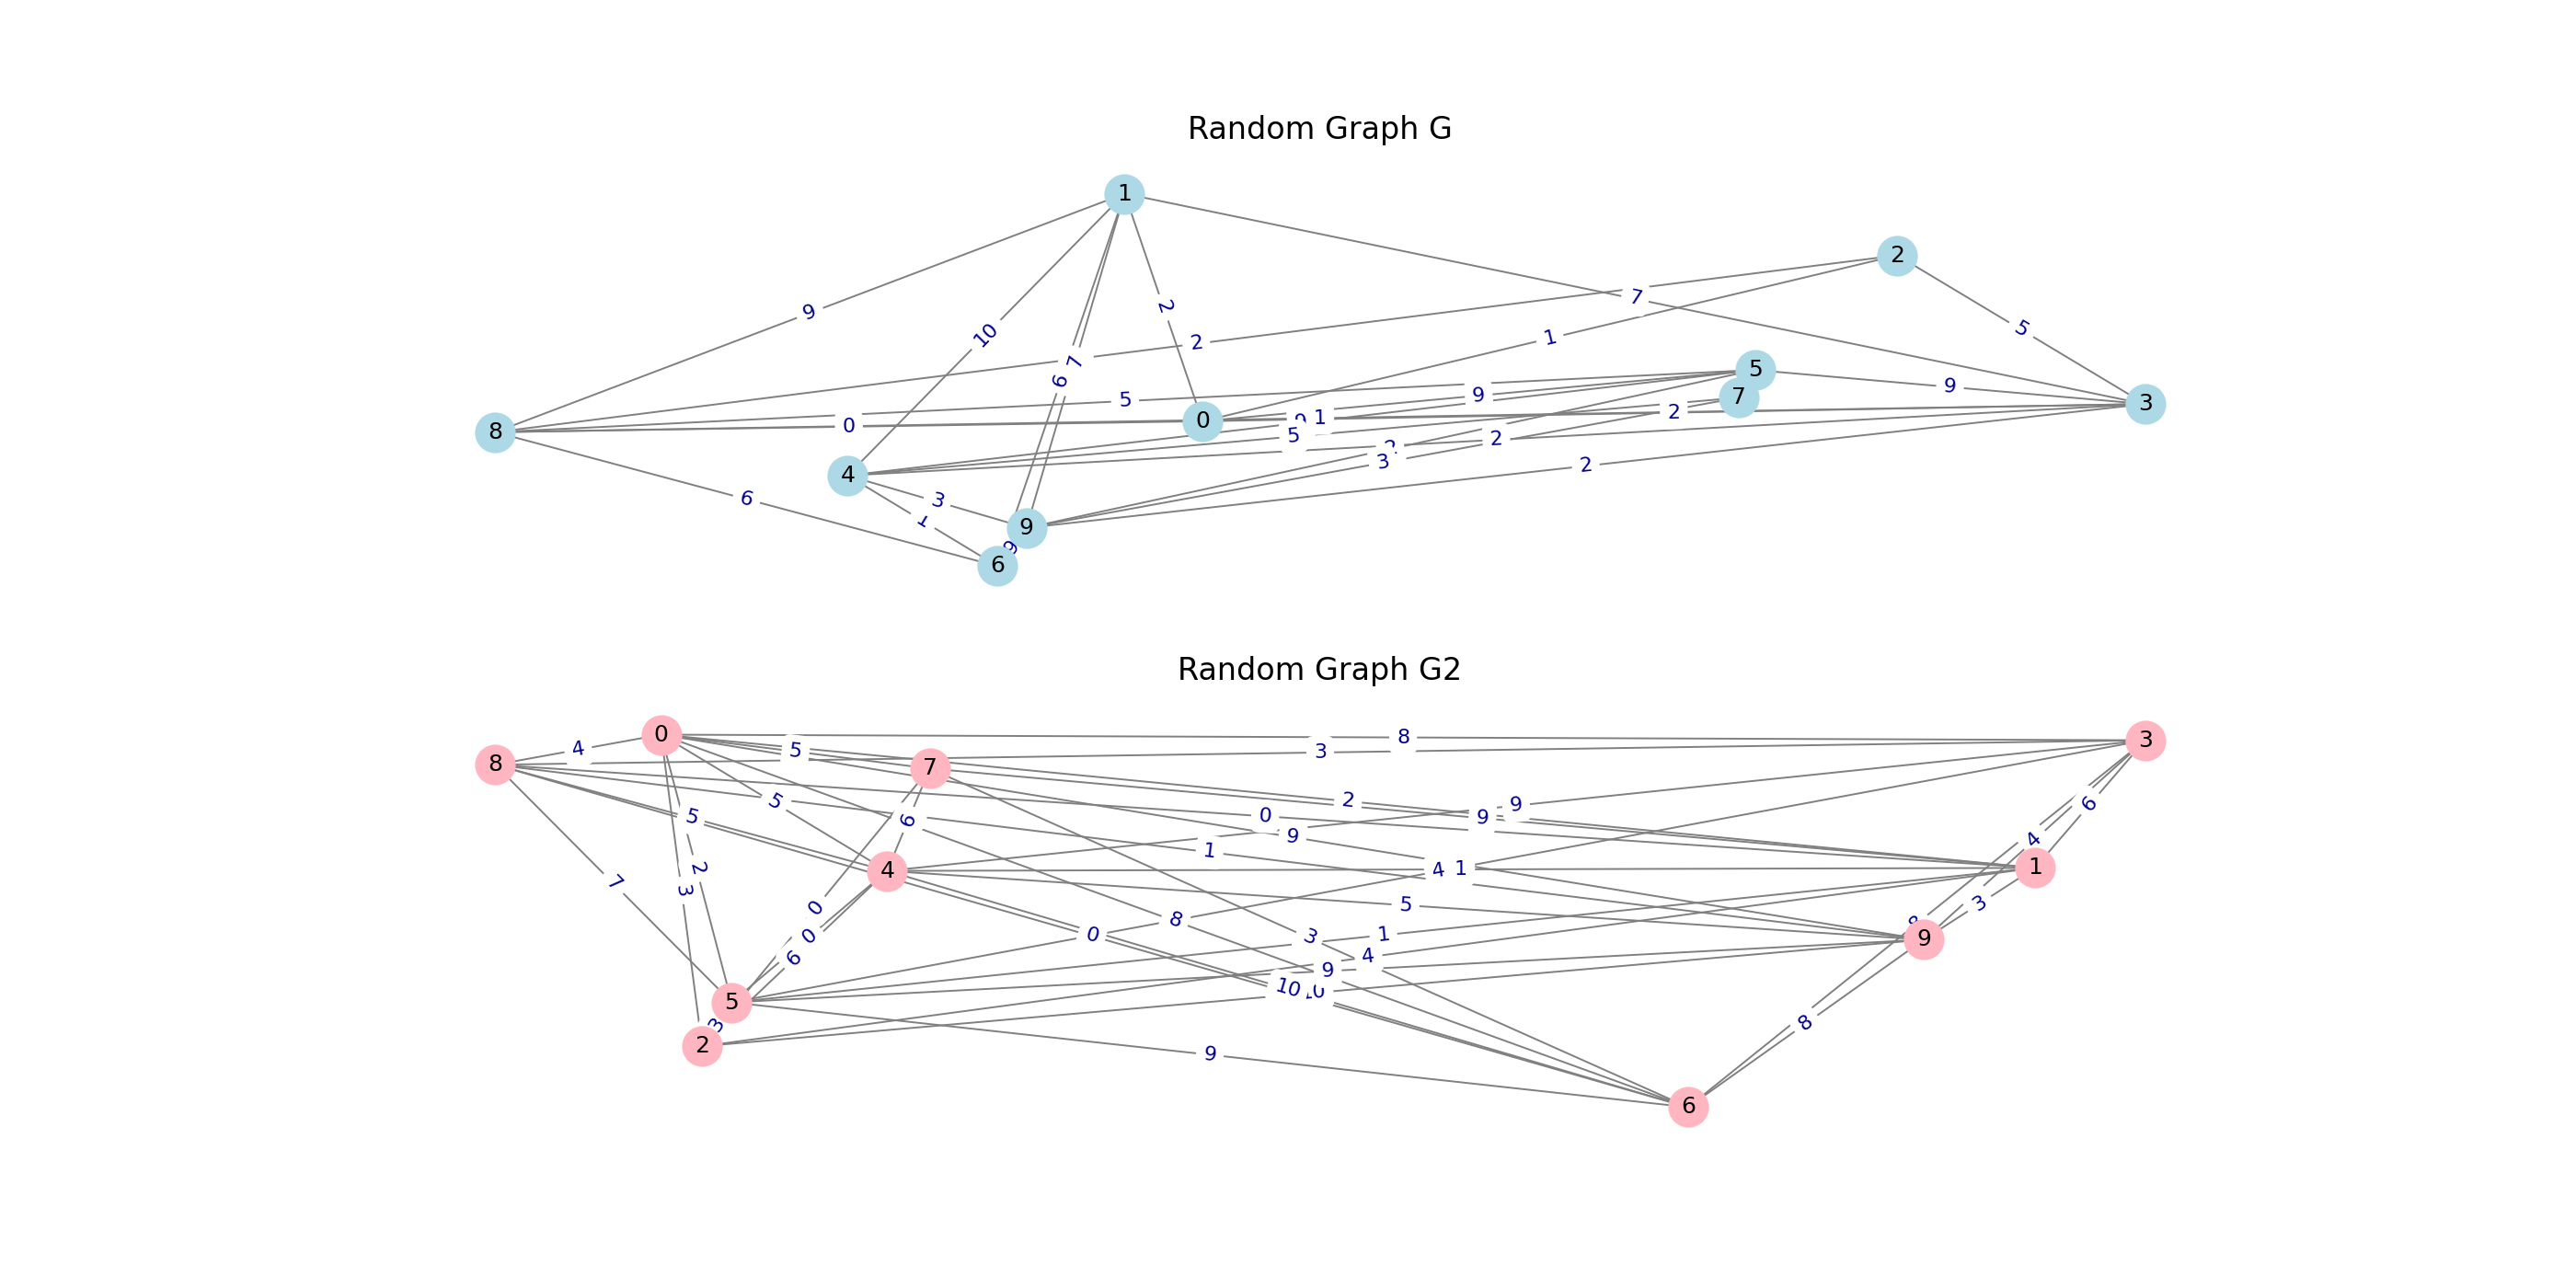
\includegraphics[width=1.0\textwidth]{Graphics/perHand2.png}
    \caption{Random Graphen-selbst implementierte Formeln}
    \label{RandomGraphenFormeln}
\end{figure}

\FloatBarrier

Nachdem der Graph \ref{RandomGraphenFormeln} leider keinesfalls einem social Network Graphen ähnelt, ist das Ziel nach wie vor, diese so gut wie möglich nachzustellen. Daher musste der Code erneut optimiert werden. Dieses mal legen wir die Hoffnung in die Darstellung durch Adjazenzmatrizen. Wie in dem ersten Teil dieser Arbeit bereits eingeführt, dürfen Netzwerke als Adjazenzmatrix dargestellt werden. In diesem Fall wurde das Programm umgeschrieben, dass es möglich ist $n$ beliebig viele Adjazenzmatrizen zu erstellen und random also zufällig zu befüllen. Anschließend werden die random befüllte Matrizen zu einem großen Graphen zusammengeführt. D.h es werden beliebig viele einzelne Matrizen zu einer ganz großen Matrix verschmolzen. Jedoch ist davor noch wichtig, den Knoten mit der größten Gradzentralität herauszufinden um an dieser Stelle die Verbindung / Brücke zu einem anderen Teilgraphen herzustellen. Dies geschieht, indem reihen- und spaltenweise Einträge der Matrix gezählt werden. Die Zeile der jeweiligen Matrizen, in der die meisten Einträge (also Werte ungleich null) stehen, wird dann als Knoten verwendet, um die anderen Teilgraphen zu verknüpfen. Der Code kann beliebig fortgeführt werden. Durch unsere Anpassungen erhalten wir nun folgenden Graphen:

\FloatBarrier
\begin{figure}[h!]
    \centering
    \hspace*{-1.5cm}
    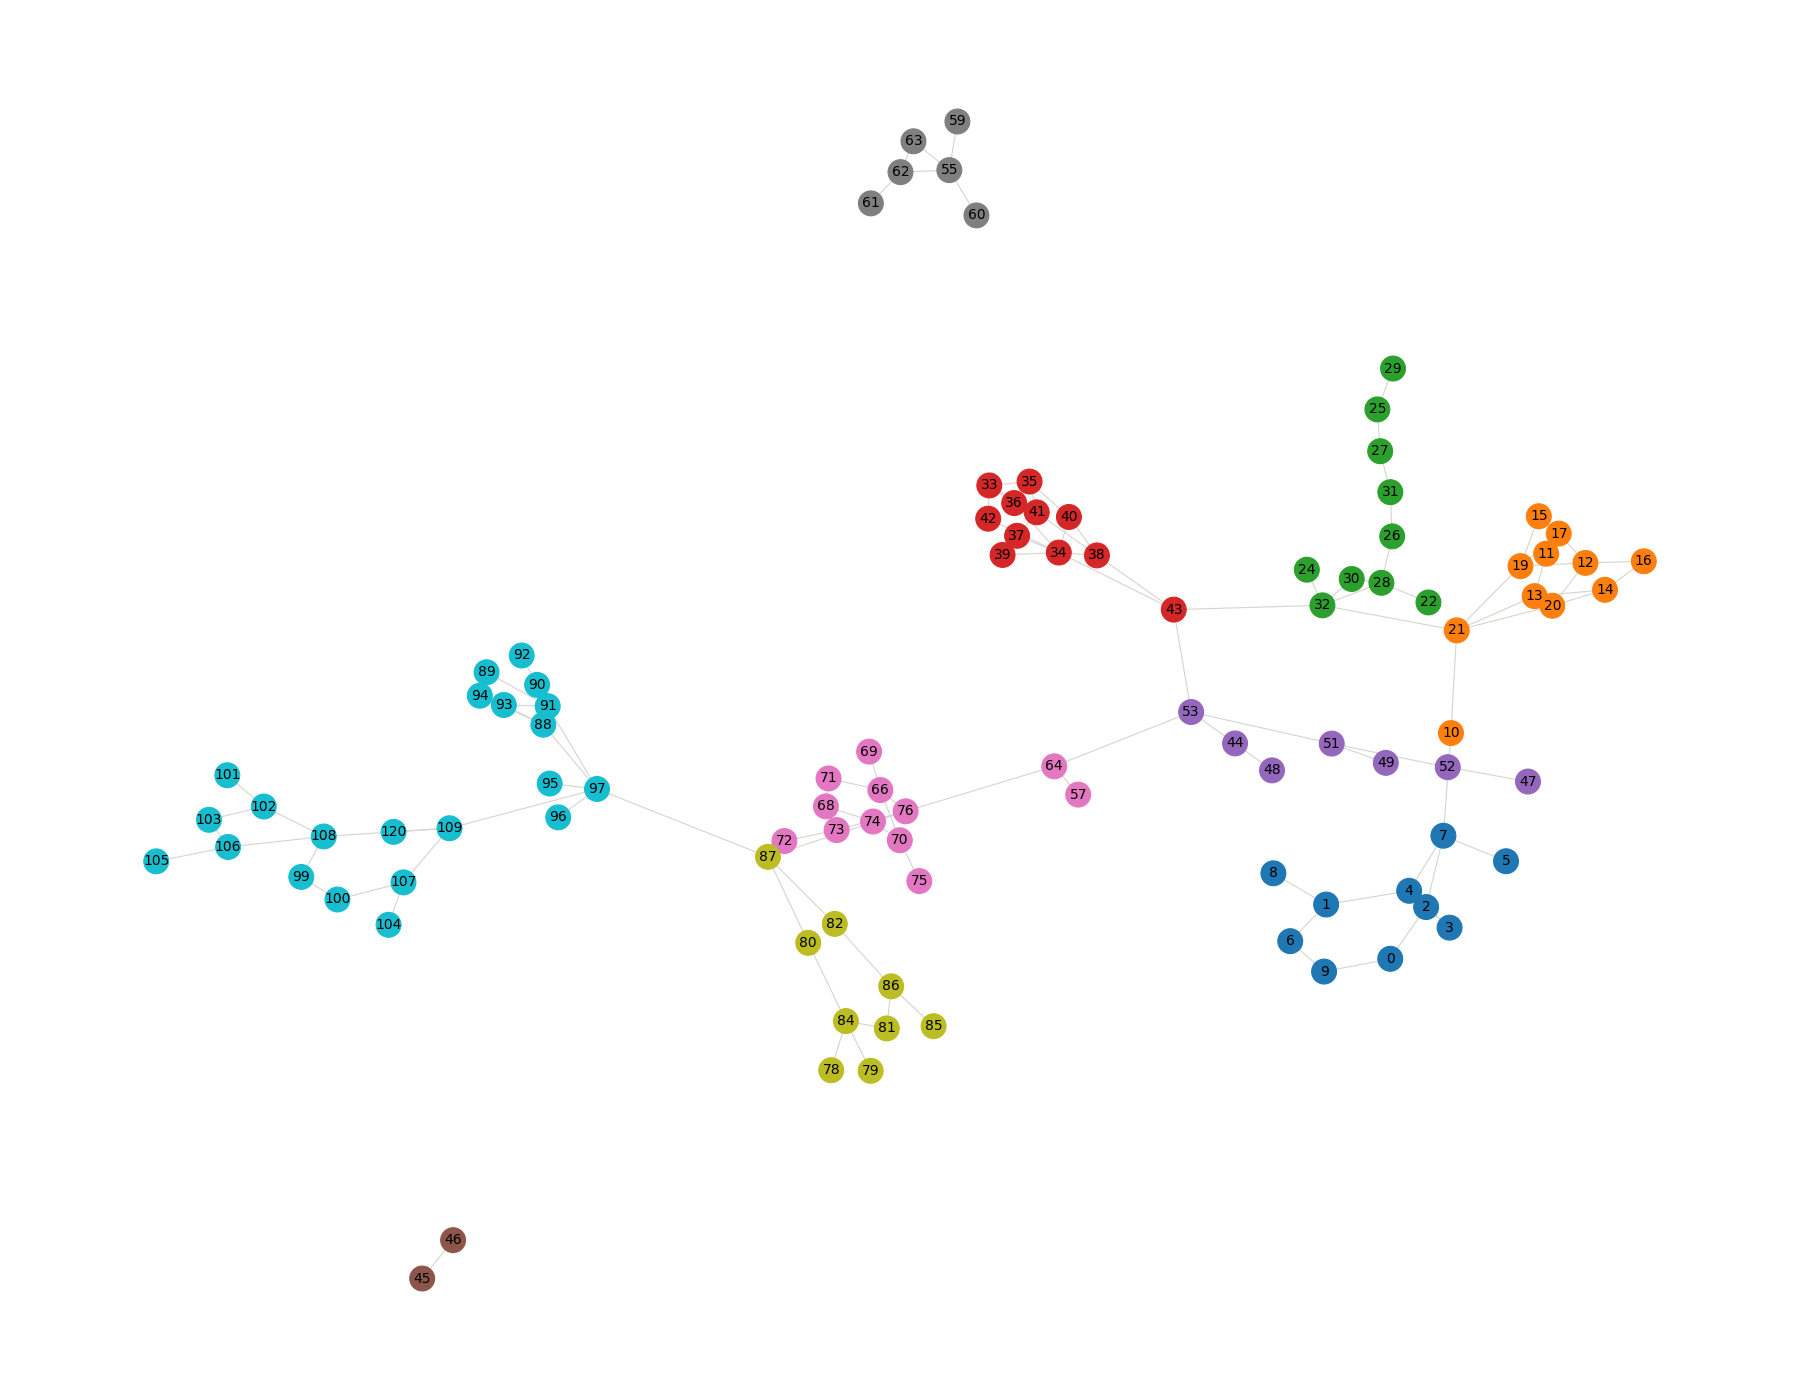
\includegraphics[width=1.2\textwidth]{Graphics/NearSocialNetwork.png}
    \caption{Random Soziale Graphen mit den höchsten Gradzentralitäts-Knoten als Verbindung }
    \label{NearSozialerGraph}
\end{figure}

Doch auch dieses Ergebnis ist nicht zufriedenstellend.
Nachdem die aktuellen Plots durchaus Sozialen Netzwerken ähneln und die Werte der Berechnungen ebenfalls richtig erscheinen, stört dennoch eine Tatsache. Bei der genaueren Betrachtung fällt auf, dass die Verbindungen untereinander, also in den kleineren Gruppen bzw. Teilgraphen, durchaus realistisch erscheinen. Jedoch wird die Möglichkeit ausgeschlossen, dass Teilgraphen verstärkt untereinander Verbindungen aufweisen. Dies liegt an der ersten Idee, den Knoten mit der höchsten Gradzentralität zu wählen und diesen dann mit einer beliebigen weiteren Gruppe zu verbinden. Doch in der Realität ist ein solches Phänomen sehr unwahrscheinlich. Denn in der Realität würde das heißen, dass beispielsweise an der Universität Ulm alle Student(en)*innen der Fakultät für Ingenieurwissenschaften, Informatik und Psychologie untereinander in einer Weise miteinander verbunden sind, jedoch nur die Professor(en)*innen, welche die höchste Gradzentralität aufweisen, mit eine*m/r weiteren Professor*in einer anderen Fakultät verbunden sind. Dies ist aber nicht realistisch wenn bedacht wird, dass auch beispielsweise Student(en)*innen der Fakultät für Mathematik und Wirtschaftswissenschaften durchaus Kontakte zu der Fakultät für Ingenieurwissenschaften, Informatik und Psychologie haben können oder auch mit den jeweiligen Professor(en)*innen. Dementsprechend müssen diese Eigenschaft ebenfalls in der Implementierung berücksichtigt werden. Dies kann gewährleistet werden indem jedem Knoten eine zufällige Wahrscheinlichkeit zugeschrieben wird, die angibt, ob eine Kante existiert, die außerhalb des definierten Bereichs, beispielsweise einer bestimmten Fakultät, liegt. Für ein gutes soziales Netzwerk muss möglich sein, dass Knoten mit vielen anderen Knoten aus anderen Teilgruppen verbunden sind. 

\section{Der endgültige optimierte Graph und die Analyse}
Mit den Überlegungen und implementierten Methode aus dem vorherigen Kapitel, lässt sich gut realisieren, dass wir einen annäherndes soziales Netzwerk erhalten:

\FloatBarrier
\begin{figure}[h!]
    \centering
    \hspace*{-2cm}
    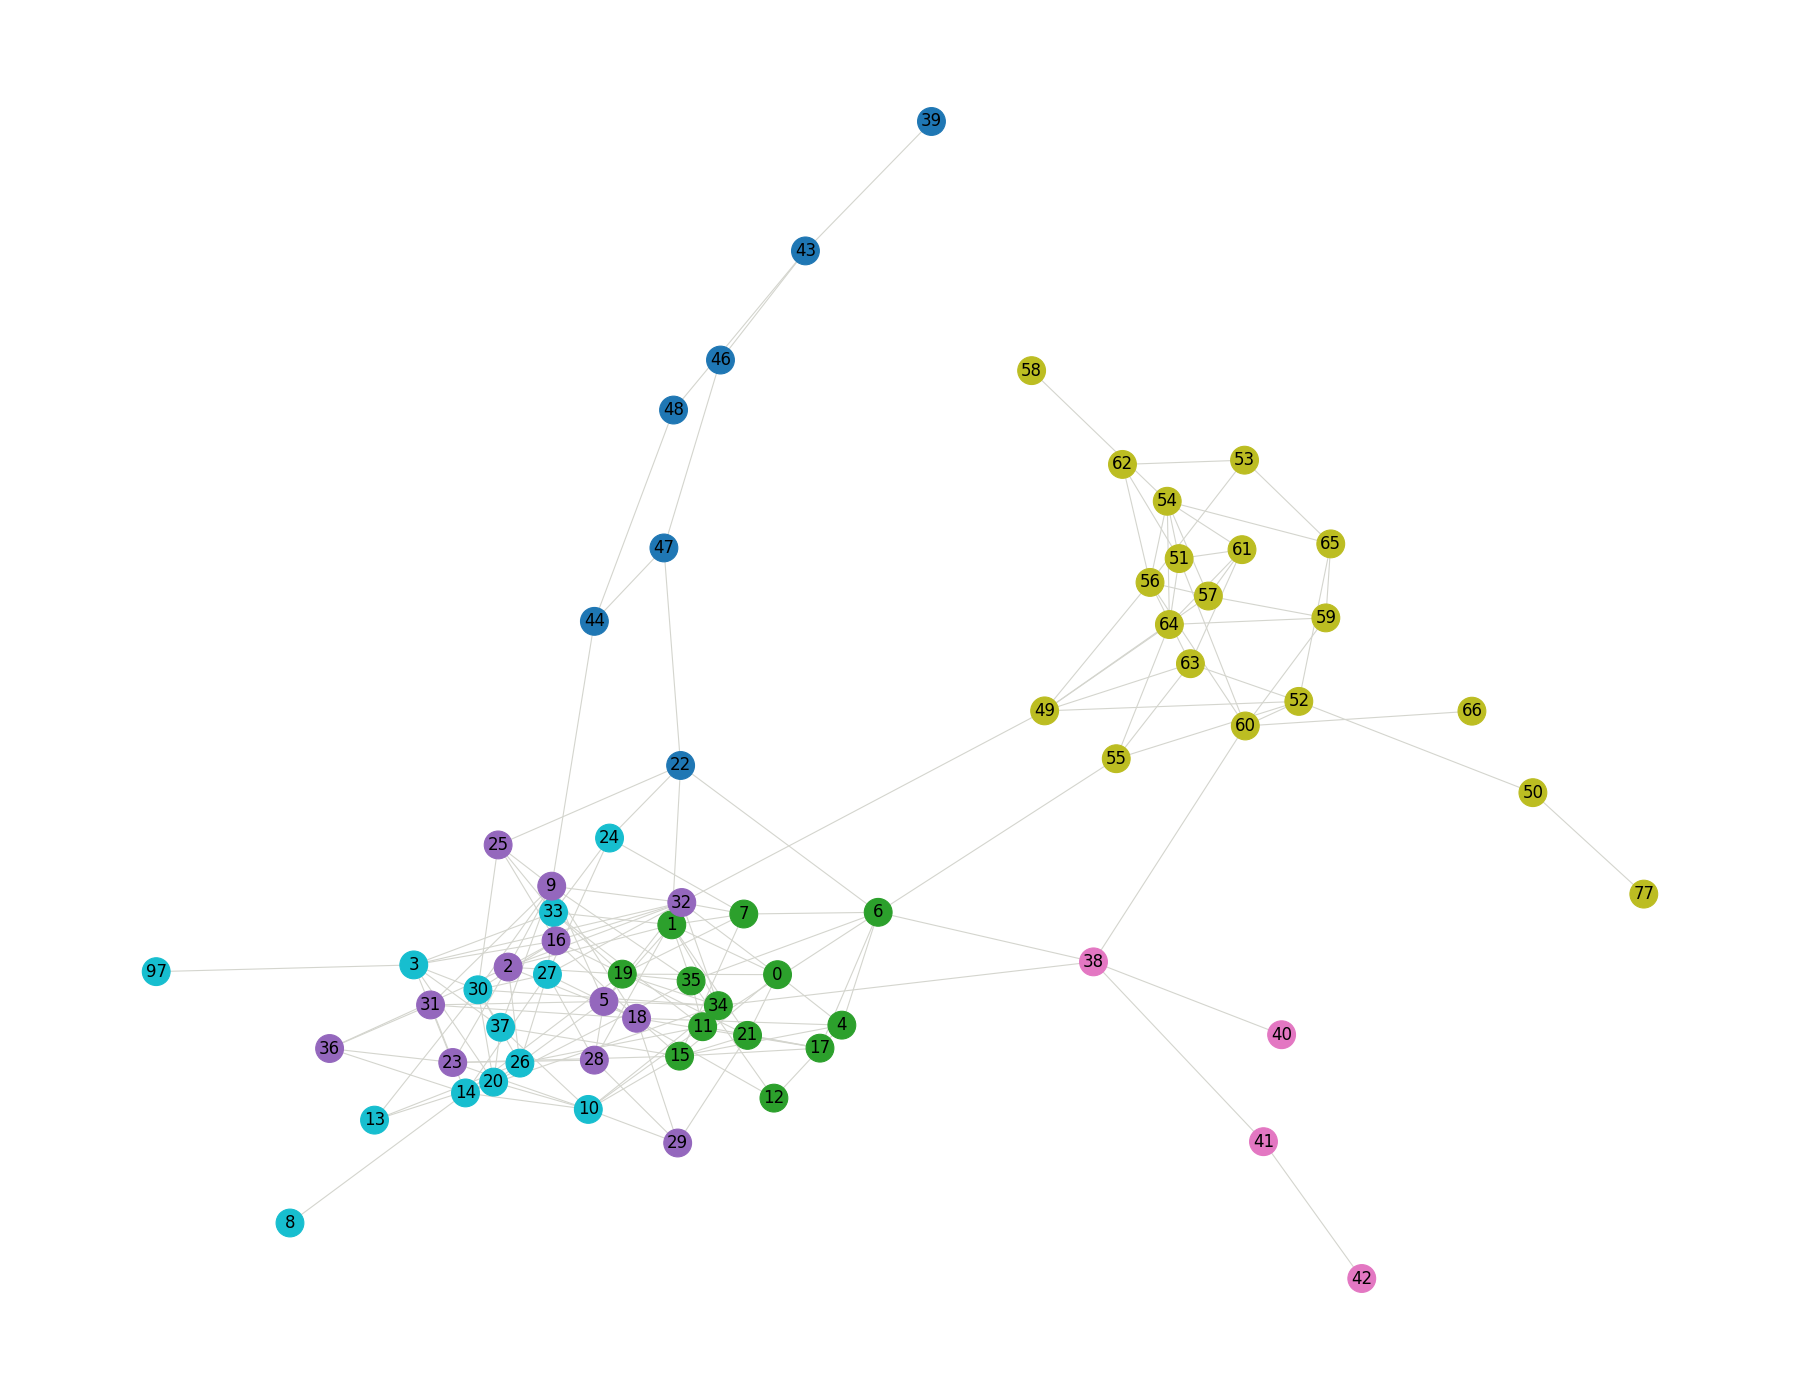
\includegraphics[width=0.9\textwidth]{Graphics/Random_moreConnections.png}
    \caption{Random soziales Netzwerk mit realistischeren Verbindungen}
    \label{fig:SNA}
\end{figure}

\FloatBarrier
Um diesen Plot zu erhalten haben wir nach wie vor primär mit Adjazenzmatrizen gearbeitet, welche erneut zufällig realisiert wurden. Statt die Knoten mit der höchsten Gradzentralität als Verbindungsglied zu wählen, wird jetzt ein beliebige Knoten mit einer beliebigen Wahrscheinlichkeit gewählt. Dadurch entstehen Graphen, die Sozialen Netzwerken tatsächlich ähneln.
Doch entsprechen die erzeugten Graphen tatsächlich näherungsweise sozialen Netzwerken? Wie kann dies bestmöglich untersucht werden?
Nachdem nun viele Faktoren optimiert sind, betrachten wir den erstellen Graphen und untersuchen diesen, ob es sich um ein soziales Netzwerk handelt.
Bei der objektiven Betrachtung des Plots ähnelt die Struktur auf jeden Fall der, eines sozialen Netzwerks. Doch um eine fundierte Aussagen treffen zu können, müssen die Zentralitäten erst genauer analysiert werden. Hierfür wird folgende Tabelle verwendet:

\begin{table}[h!]
\footnotesize
\caption{Werte oberer Graph}
\begin{tabular}{lcccc}\toprule 
\textbf{Knoten} &\textbf{Grad-Zentr.} &\textbf{Nähe-Zentr.}  &\textbf{Between-Zentr.} \\
 &\\\midrule
  1 & 0.149254  & 0.389535 & 0.0429244   \\
  2 & 0.134328  & 0.370166 & 0.0366434   \\
  3 & 0.119403  & 0.350785 & 0.0516569   \\
  5 & 0.119403  & 0.378531 & 0.0341306   \\
  6 & 0.119403  & 0.385057 & 0.145038    \\
  7 & 0.0895522 & 0.358289 & 0.0208983   \\
 10 & 0.119403  & 0.341837 & 0.0240985   \\
 11 & 0.104478  & 0.360215 & 0.0212421   \\
 14 & 0.119403  & 0.3350    & 0.0454434   \\
 18 & 0.134328  & 0.340102 & 0.0283754   \\
 22 & 0.0746269 & 0.348958 & 0.0740623   \\
 27 & 0.119403  & 0.360215 & 0.0342121   \\
 30 & 0.149254  & 0.348958 & 0.0412278   \\
 32 & 0.179104  & 0.435065 & 0.266448    \\
 34 & 0.134328  & 0.394118 & 0.112543    \\
 35 & 0.104478  & 0.362162 & 0.0290967   \\
       
  \\\bottomrule
 \end{tabular}
  &
\begin{tabular}{lccc}
\toprule 
\textbf{Knoten} &\textbf{Grad-Zentr.} &\textbf{Nähe-Zentr.}  &\textbf{Between-Zentr.}\\
   &\\\midrule
 38 & 0.0746269 & 0.36612  & 0.154688    \\
 41 & 0.0298507 & 0.271255 & 0.0298507   \\
 43 & 0.0447761 & 0.198813 & 0.030303    \\
 44 & 0.0447761 & 0.295154 & 0.0773717   \\
 46 & 0.0298507 & 0.219672 & 0.0205638   \\
 47 & 0.0447761 & 0.27459  & 0.0520902   \\
 48 & 0.0298507 & 0.232639 & 0.0373285   \\
 49 & 0.0895522 & 0.36413  & 0.221288    \\
 50 & 0.0298507 & 0.241877 & 0.0298507   \\
 52 & 0.0895522 & 0.314554 & 0.0885577   \\
 54 & 0.104478  & 0.254753 & 0.0327816   \\
 55 & 0.0597015 & 0.325243 & 0.0670173   \\
 56 & 0.104478  & 0.303167 & 0.0672381   \\
 57 & 0.0746269 & 0.290043 & 0.0213757   \\
 60 & 0.0895522 & 0.313084 & 0.0903114   \\
 64 & 0.0895522 & 0.304545 & 0.0530434   \\
      \\\bottomrule
\end{tabular}
\end{table}
\label{TablleSNA}

Bei dieser Tabelle handelt es sich um die \textbf{32} wichtigsten Knoten. Die Anzahl der Knoten in der Tabelle \ref{TablleSNA} ist rein zufällig gewählt und hat keine Bedeutung. Alle Knoten die eine geringere \textbf{"Betweenness-Centrality"} kleineren als \textbf{0.02} aufweisen, sind außen vor gelassen. Auch hier haben wir die Grenze rein zufällig gewählt. Bei diesem Grenzwert handelt es sich um einen guten Mittelwert. Wir wollen weder zu wenig, noch zu viele Knoten betrachten. Doch betrachten wir nun die Tabelle \ref{TablleSNA} genauer. 
Bei der Grad-Zentralität sehen wir, dass die meisten Knoten einen Wert höher als \textbf{0.1} aufweisen. Wir können einen Schritt weitergehen und stellen schnell fest, dass einige wenige Knoten eine Grad-Zentralität höher als \textbf{0.13} aufweisen. Genau genommen handelt es sich hier um die Knoten \textbf{1} mit einem Wert von \textbf{0.149254}, den Knoten \textbf{2} mit dem Wert \textbf{0.134328}, Knoten \textbf{18} mit dem Wert \textbf{0.134328}, dann Knoten \textbf{30} mit einer Zentralität von \textbf{0.149254}, zudem um den Knoten \textbf{32} mit dem höchsten Wert von \textbf{0.179104} und schließlich Knoten \textbf{34} mit einer Grad-Zentralität von \textbf{0.134328}. All diese aufgezählten Knoten sind zentral wichtig für den Graphen und befinden sich höchstwahrscheinlich im Zentrum des Graphen \ref{fig:SNA}. Betrachten wir nun die Abbildung genauer, kann diese Behauptung teilweise bestätigt werden, denn die Knoten stechen auf jeden Fall heraus, doch befinden sie sich nicht ganz mittig im Graphen.  Diese relativ hohen Werte sagen über die Knoten aus, dass es sich im realen Leben um eine sehr berühmte / bekannte Person handeln muss. Wir können beispielsweise annehmen, dass es ein Star, ein Influenzer oder eine, auf weitere Arten bekannte Person ist. Doch ebenso können wir annehmen, dass die Person lediglich viele andere Personen kennt, oder von vielen anderen Personen gekannt wird. Doch nicht nur die Grad-Zentralität spielt für uns und die Analyse in dieser Arbeit eine zentrale Rolle. Im Weiteren betrachten wir die \textbf{"Nähe-Zentralität"} doch um auch bei diesem Aspekt nicht alle \textbf{32} Werte aufzuzählen, betrachten wir im Folgenden nun Knoten, die einen Wert höher als \textbf{0.37} aufzeigen. Hierzu zählen der Knoten \textbf{1} mit einem Wert von \textbf{0.389535}, Konten \textbf{2} mit dem Wert \textbf{0.370166}, zudem Knoten \textbf{5} mit dem Wert \textbf{0.378531}, zusätzlich Knoten \textbf{6} mit der Zentralität \textbf{0.385057}, und schließlich die Knoten \textbf{32} mit dem höchsten Wert \textbf{0.435065} und \textbf{34} mit der Zentralität von \textbf{0.394118}. Je höher die Werte sind, so haben wir in dem ersten Teil der Arbeit gesehen, desto näher Befinden sich diese Knoten zu weiteren bzw. weisen die durchschnittlich kürzesten Wege nach. Betrachten wir nach dieser Information unseren Graphen \ref{fig:SNA} und suchen die Knoten mit der höchsten \textbf{Nähe-Zentralität}, sehen wir direkt, dass sich diese im gleichen Bereich befinden, wie die Knoten mit der höchsten \textbf{Grad-Zentralität}. Doch bestätigt der Plot unsere Vermutung nicht eindeutig, da es teilweise nicht ideal zu erkennen ist, ob die Kanten zum Knoten verlaufen oder an diesem vorbei. Doch diese Problematik ist nicht neu für uns, sie ist bereits im ersten Teil bei der Analyse des \textbf{Game of Thrones} Graphen \ref{fig:GameOfThrones} aufgetreten. Wobei auch die Möglichkeit besteht, dass wir die Formeln nicht korrekt implementiert haben. Jedoch hat händisches Nachrechnen, bei durchaus kleineren Plots, die Korrektheit ergeben, weshalb wir diese Vermutung in Klammern setzen und uns eher auf die nicht eindeutigen Darstellung einigen. Doch nun kommen wir zur letzten untersuchten Zentralität, nämlich der \textbf{Betweenness-Zentralität}. Auch hier betrachten wir wieder die Knoten mit den höchsten Werten, und um nicht alle \textbf{32} Werte aufzuzählen, betrachten wir erneut nur Knoten mit einem Wert höher als \textbf{0.09}. Diese Voraussetzung erfüllen neben dem Knoten \textbf{6} mit dem Wert \textbf{0.145038} die Knoten \textbf{32} mit der höchsten Zentralität von \textbf{0.266448} und \textbf{34} mit einem Wert von \textbf{0.112543}, außerdem der Knoten \textbf{38} mit der Zentralität von \textbf{0.154688}, zudem der Knoten \textbf{49} mit dem Wert \textbf{0.221288} und schließlich der Knoten \textbf{60} mit dem Wert \textbf{0.0903114}. Das bedeutet für unseren Graphen \ref{fig:SNA}, dass die kürzesten Wege anteilsmäßig am öftesten über diese genannten Knoten verlaufen. Betrachten wir erneut den Graphen, sehen wir eine zum Teil bekannte Eigenschaft, dass sich die Punkte im grün, lila, hellblau verschmolzenen, links unten zentrierten, drei Teilgraphen befinden. Doch kommt bei der \textbf{Betweenness-Zentralität} hinzu, dass sich die Knoten \textbf{49 und 60} auch im gelbgrünen, rechts oben liegenden, Teilgraphen befinden. In diesem Fall sehen wir sogar schön, dass die Werte gut zu unserem Plot passen und es sehr wahrscheinlich ist, dass unsere Annahme korrekt ist, und die Knoten tatsächlich am häufigsten bei allen kürzesten Wegen durchlaufen werden. Weitere Zentralitätswerte müssen wir nicht betrachten. Zum einen gäbe es hier noch die \textbf{Eigenvektor-Zentralität}, doch würde diese nur unsere Feststellungen bestätigen. Jetzt haben wir alle Kriterien überprüft und erfolgreich festgestellt, dass dieser Graph einem \textbf{sozialen Netzwerk} ähnelt. Doch um auszuschließen, dass wir hier rein zufällig ein solches erhalten haben, möchten wir uns noch ein weiteres Kriterium überlegen und anschließend untersuchen.


\section{Die Verteilung der Zentralitäten}
Nachdem wir im vorherigen Kapitel eine \textbf{soziale Netzwerkanalyse} durchgeführt haben und ein gutes soziales Netzwerk künstlich generiert haben, möchten wir uns im Folgenden die Verteilung der Zentralitätswerte anschauen.
Im Laufe der Arbeit ist aufgefallen, dass sich die Werte der Zenralitäten oftmals in ähnlichen Bereichen befinden. An dieser Stelle können wir uns die Frage stellen, wie diese Werte verteilt sind. Vielleicht existieren Zusammenhänge zwischen unseren generierten sozialen Netzwerken und sozialen Netzwerken im Allgemeinen. Das heißt, im Konkreten, wollen wir der Frage nachgehen, ob alle Zentralitätswerte sozialer Netzwerke ähnliche Verteilungen nachweisen. Würde sich unsere Vermutung diesbezüglich bestätigen, können wir andere soziale Netzwerke anhand dieses Kriterium untersuchen und interessante Vermutungen aufstellen. Zunächst aber implementieren wir die Methode, die die Verteilung der Zentralitäten untersucht anhand der \textbf{Gradzentralität}.
Da der Graph \ref{fig:SNA} ein zufällig, einmalig erzeugter Graph ist, werden wir nicht einen Identischen Graphen erzeugen können, um die Verteilung der Zentralitäten zu betrachten. Was sich jedoch nicht negativ auf die weiteren Untersuchungen auswirken sollte. Den ersten Graphen und die zugehörige Verteilung der Gradzentralität bildet sich folgendermaßen ab: 

\FloatBarrier
\begin{figure}[h!]%
  \centering
  \subfloat[][]{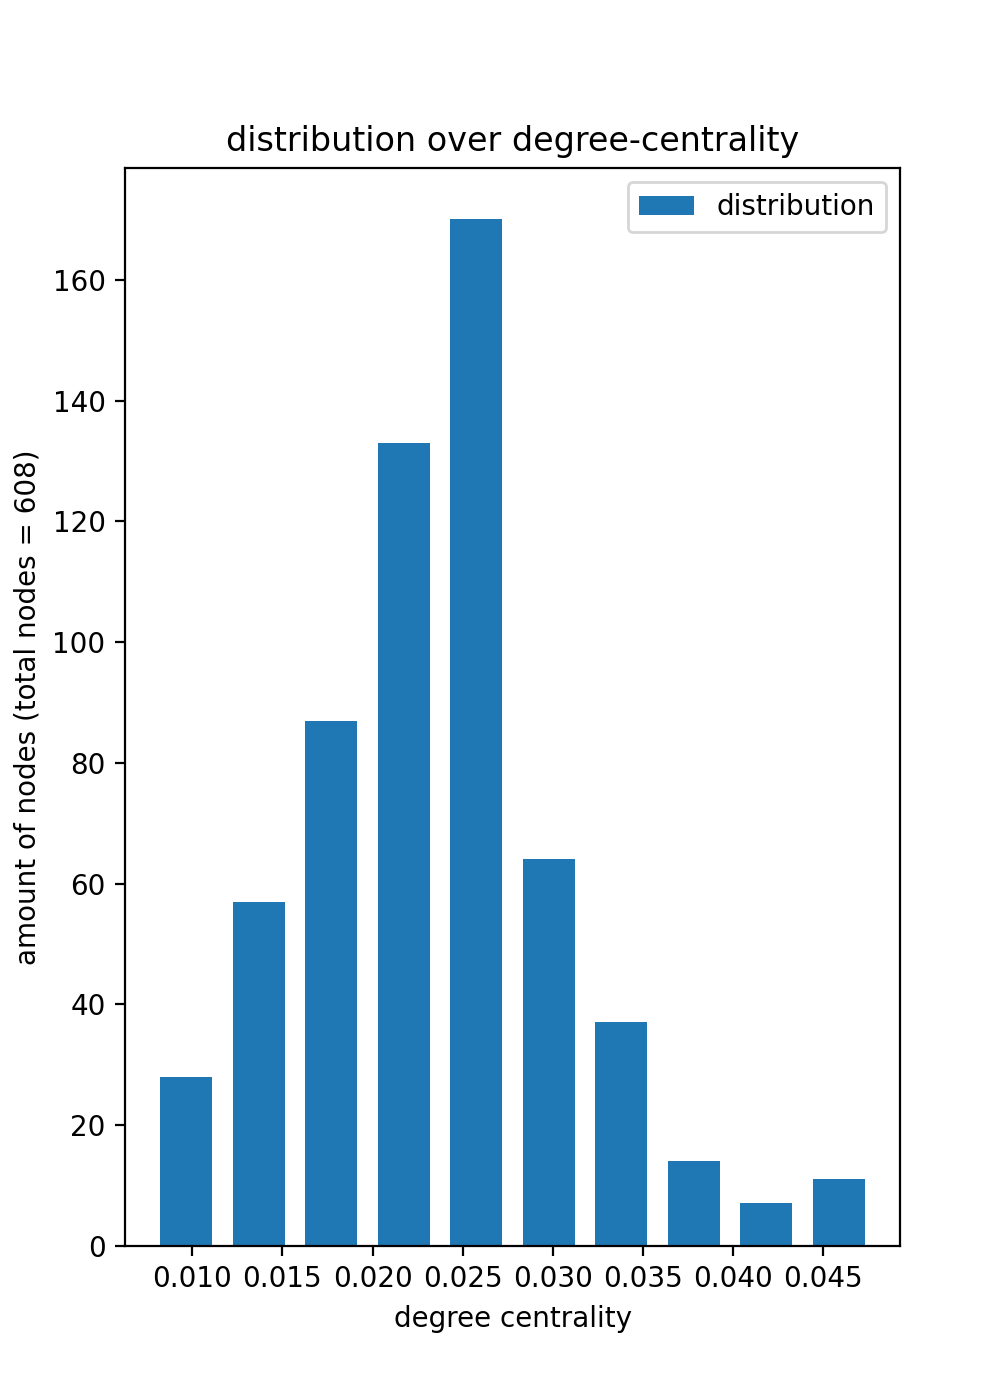
\includegraphics[width=0.4\linewidth]{Graphics/distribution_degree.png}}%
  \qquad
  \subfloat[][]{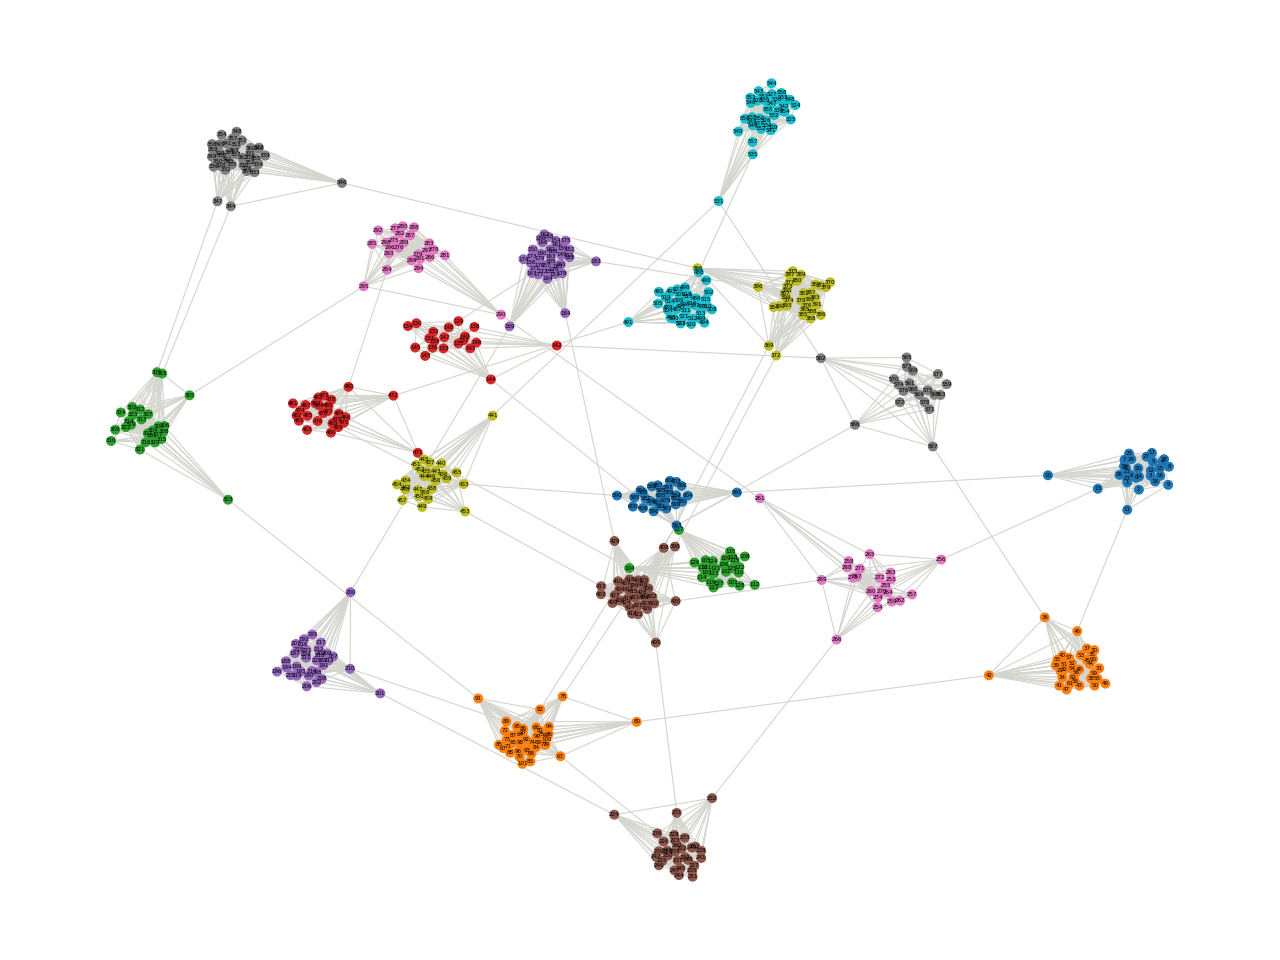
\includegraphics[width=0.5\linewidth]{Graphics/plot_degreeDist.png}}%
  \caption{Verteilung der Grad-Zentralität des Graphen (b)}%
  \label{fig:distribution}
\end{figure}

\FloatBarrier
Jedoch ist zu erwähnen, dass wir keine perfekte Gauß-Verteilung generieren, sondern eine etwas nach links verschobene Verteilung sehen. An was dies liegen kann, werden wir uns später anschauen und versuchen das Phänomen zu analysieren. Nun wollen wir untersuchen, ob sich die Eigenschaft, der gleichmäßig verteilten Zentralitäten für die \textbf{Nähe-} und \textbf{Betweenness-Zentralität} bestätigt. 
